
In the previous section we derived differential equations that model mechanical, electrical, and electro-mechanical systems.  The equations themselves often do not provide sufficient information.  For example, we were able to find a signal $p$ representing the position of the mass-spring-damper in Figure~\ref{mech:massspring1} given a particular force signal $f$ is applied to the mass.  However, it is not immediately obvious how to find the force signal $f$ given a particular position signal $p$.  We will be able to solve this problem and, more generally, to describe properties of systems modelled by linear differential equations with constant coefficient, if we make the added assumptions that the systems are \term{linear} and \term{shift-invariant}.  We study linear shift-invariant systems in this chapter.  %Throughout this chapter $H$ will denote a linear shift-invariant system.

\section{Convolution, regular systems and the delta ``function''} \label{sec:conv-regul-syst}

A large number of linear shift-invariant systems can be represented by a signal called the \term{impulse response}.  The impulse response of a system $H$ is a locally integrable signal $h$ such that
\[
Hx(t) = \int_{-\infty}^{\infty} h(\tau) x(t - \tau) d\tau,
\]
that is, the response of $H$ to input signal $x$ can be represented as an integral equation involving $x$ and the impulse response $h$.  The integral is called a \term{convolution} and appears so often that a special notation is used for it.  We write $h * x$ to  indicate the signal that results from convolution of signals $h$ and $x$, that is, $h * x$ is the signal
\[
h * x = \int_{-\infty}^{\infty} h(\tau) x(t - \tau) d\tau
\]
where the right hand side is to be interpreted as a signal, a function of $t \in \reals$.  We write $(h*x)(t)$ to indicate the value of $h*x$ at $t \in \reals$.  
Those systems that have an impulse response we call \term{regular systems}\footnote{The name \term{regular system} is motivated by the term \term{regular distribution}~\citep{Zemanian_dist_theory_1965}}.  

Some care must be taken when selecting a domain for a regular system.  To see what can go wrong it is worth first considering an example.  Suppose that $H$ has discrete impulse response given by the step function $u$~\eqref{eq:stepfunction}.  The signal $x(t) = 1$ that takes the value $1$ for all $t \in \reals$ will not be in the domain of $H$ since, in this case,
\[
Hx(t) =  \int_{-\infty}^{\infty} u(\tau) x(t - \tau) d\tau = \int_{0}^{\infty} d\tau
\]
is not finite for any $t \in \reals$.  Given a signal $h$, denote by $\dom h$ the set of signals $x$ such that the integral
\[
\int_{-\infty}^{\infty} \abs{h(\tau) x(t - \tau)} d\tau < \infty \qquad \text{for all $t \in \reals$}.
\]
If $H$ has impulse reponse $h$ then, for all signal $x \in \dom h$ we have
\[
\abs{Hx(t)} = \abs{\int_{-\infty}^{\infty} h(\tau) x(t - \tau) d\tau} \leq \int_{-\infty}^{\infty} \abs{h(\tau) x(t - \tau)} d\tau < \infty 
\]
for all $t \in \reals$ and so $Hx(t)$ is finite for all $t \in \reals$.  We take $\dom h$ as the domain of a regular system $H$ with impulse response $h$ unless otherwise stated.  It can be shown that $\dom h$ is a linear shift-invariance space (Exercise~\ref{exer:finhlinshiftinv}).

Regular systems are linear because, for all $x, y \in \dom h$ and all $a, b \in \complex$,
\begin{equation}\begin{split}\label{eq:regsystemislinear}
H(ax + by) &= h * (ax + by) \\
&= \int_{-\infty}^{\infty} h(\tau) \big(ax(t - \tau) + by(t - \tau)\big) d\tau \\
&= a\int_{-\infty}^{\infty} h(\tau) x(t - \tau) d\tau + b\int_{-\infty}^{\infty} h(\tau)y(t - \tau) d\tau \\
&= a (h * x) + b(h*y) \\
&= a Hx + bHy.
\end{split}\end{equation}
The above equation shows that convolution commutes with scalar multiplication and distributes with addition, that is,
\[
h * (ax + by) =  a (h * x) + b(h*y).
\]
Regular systems are also shift-invariant because for all $x \in \dom h$
\begin{align*}
T_\kappa H x &= T_\kappa(h * x ) \\
&= \int_{-\infty}^{\infty} h(\tau) x(t- \kappa - \tau) d\tau \\
&= \int_{-\infty}^{\infty} h(\tau) T_\kappa x(t - \tau) d\tau \\ 
&= h * (T_\kappa x) \\
&= H T_\kappa x. 
\end{align*}

The impulse response of a regular system $H$ can be found in the following way.  First define the signal
\[
p_\gamma(t) = \begin{cases}
\gamma, & 0 < t \leq \frac{1}{\gamma} \\
0, & \text{otherwise},
\end{cases}
\]
that is, a rectangular shaped pulse of height $\gamma$ and width $\tfrac{1}{\gamma}$.  The signal $p_\gamma$ is plotted in Figure~\ref{fig:rectpulsedelta} for $\gamma=\frac{1}{2},1,2,5$.  As $\gamma$ increases the pulse gets thinner and higher so as to keep the area under $p_\gamma$ equal to one.  Consider the response of the regular system $H$ to the signal $p_\gamma$,
\begin{align*}
H p_\gamma = h * p_\gamma = \int_{-\infty}^\infty h(\tau) p_\gamma(t - \tau) d\tau = \gamma \int_{t- 1/\gamma}^{t} h(\tau) d\tau.
\end{align*}
Taking $\gamma \to \infty$ we find that
\[
\lim_{\gamma \rightarrow \infty} H p_\gamma = \lim_{\gamma \rightarrow \infty} \gamma \int_{t- 1/\gamma}^{t} h(\tau) d\tau = h \;\; \text{a.e.}
\]
%that is, the impulse response satisfies $h = \lim_{\gamma \rightarrow \infty} H p_\gamma$ almost everywhere.  %If this limit does not converge for any $t$, then the system is not regular and does not have an impulse response.  %The reader unclear on the meaning of the limit above might want to review Section~\ref{sec:convergence-signals}.

%BLERG Young's inequality gives a neat way of knowing when convolutions exist or don't exists based on what Lp space the signals lie in.  This becomes useful in the Fourier transform section?

As an example, consider the integrator system $I_\infty$ described in Section~\ref{sec:some-import-syst}.  The response of $I_\infty$ to $p_\gamma$ is 
\[
I_\infty p_\gamma(t) = \int_{-\infty}^{t} p_\gamma(\tau) d\tau = \begin{cases}
0, & t \leq 0 \\
\gamma t, & 0 < t \leq \frac{1}{\gamma} \\
1, & t > \frac{1}{\gamma}.
\end{cases}
\]
The response is plotted in Figure~\ref{fig:rectpulsedelta}.  Taking the limit as $\gamma \rightarrow\infty$ we find that the impulse response of the integrator is the step function
\begin{equation}\label{eq:utimprespstep}
u(t) = \lim_{\gamma\rightarrow\infty} H p_\gamma(t) = \begin{cases}
0 & t \leq 0 \\
1 & t > 0.
\end{cases} \qquad \text{a.e.}
\end{equation}

\newcommand{\rectpulse}[1]{\draw[color=black,thick] (-0.5,0) -- (0,0) -- (0,#1) -- (1.0/#1,#1) node[right] {$\gamma=#1$}-- (1.0/#1,0) -- (3,0)}
\newcommand{\pulseresponse}[2]{\draw[color=black,thick] (-0.5,0) -- (0,0) -- node [rotate=atan(#1),pos=#2,below] {$\gamma=#1$} (4*1.0/#1,4*1) -- (4*5,4*1)}
\begin{figure}[tp]
  \centering
  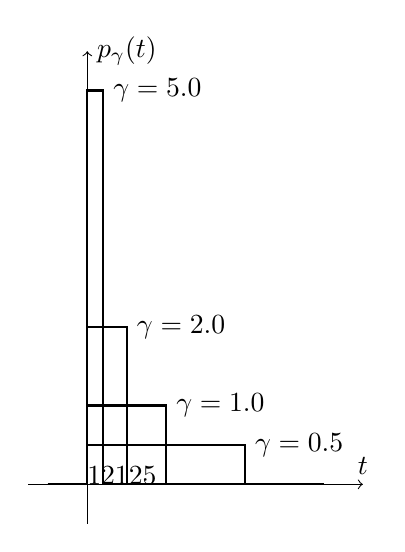
\begin{tikzpicture}
    % \draw[very thin,color=gray] (-0.1,-1.1) grid (3.9,3.9);
    \draw[->] (-0.75,0) -- (3.5,0) node[above] {$t$};
    \draw[->] (0,-0.5) -- (0,5.5) node[right] {$p_\gamma(t)$};
    \rectpulse{1.0};
    \rectpulse{5.0};
    \rectpulse{2.0};
    \rectpulse{0.5};
    \vtick{1.0} node[pos=0.5,below] {$1$};
    \vtick{2.0} node[pos=0.5,below] {$2$};
    \htick{1.0} node[pos=0.5,left] {$1$};
    \htick{2.0} node[pos=0.5,left] {$2$};
    \htick{5.0} node[pos=0.5,left] {$5$};
  \end{tikzpicture}
\;\;
  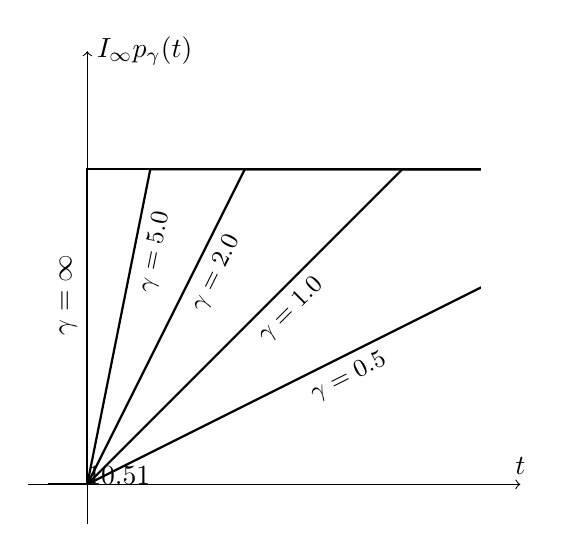
\begin{tikzpicture}
    % \draw[very thin,color=gray] (-0.1,-1.1) grid (3.9,3.9);
    \draw[->] (-0.75,0) -- (5.5,0) node[above] {$t$};
    \draw[->] (0,-0.5) -- (0,5.5) node[right] {$I_\infty p_\gamma(t)$};
    \begin{scope}[font=\small]
      \clip (0,0) rectangle (5,5);
      \pulseresponse{5.0}{0.75};
      \pulseresponse{2.0}{0.7};
      \pulseresponse{1.0}{0.6};
      \pulseresponse{0.5}{0.4};
    \end{scope}
    \draw[color=black,thick] (-0.5,0) -- (0,0) -- node[rotate=90,pos=0.6,above] {$\gamma=\infty$} (0,4) -- (5,4);
    \htick{4.0} node[pos=0.5,left] {$1$};
    \vtick{2.0} node[pos=0.5,below] {$0.5$};
    \vtick{4.0} node[pos=0.5,below] {$1$};
  \end{tikzpicture}
  \caption{The rectangular shaped pulse $p_\gamma$ for $\gamma=0.5,1,2,5$ and the response of the integrator $I_\infty$ to $p_\gamma$ for $\gamma=0.5,1,2,5,\infty$.} \label{fig:rectpulsedelta}
\end{figure}

Some important systems do not have an impulse response and are not regular.  For example, the identity system $T_0$ is not regular.  % because 
% \[
% \lim_{\gamma \rightarrow \infty} T_0 p_\gamma = \lim_{\gamma \rightarrow \infty} p_\gamma
% \]
% does not converge.  
% BLERG what is this all about actually?  Is is something like.  The convergence is not ``almost everywhere''?
Similarly, the  shifter $T_\tau$ and differentiators $D^k$ are not regular.  However, it is common to pretend that $T_0$ \emph{does} have an impulse response and this is typically denoted by the symbol $\delta$ called the \term{delta function}.  The idea is to assign $\delta$ the property
\[
\int_{-\infty}^\infty x(t) \delta(t) dt = x(0) %= \lim_{\gamma \rightarrow \infty}\int_{\infty}^\infty x(t) p_\gamma(t) dt
\]
so that convolution of $x$ and $\delta$ satisfies
\[
\delta * x = \int_{-\infty}^{\infty} \delta(\tau) x(t - \tau) d\tau = x(t) = T_0 x .
\]
We now treat $\delta$ as if it were a signal.  So $\delta(t - \tau)$ will represent the impulse response of the shifter $T_\tau$ because
\begin{align*}
T_\tau x &= \delta(t - \tau) * x \\
&= \int_{-\infty}^{\infty} \delta(\kappa -\tau) x(t - \kappa) d\kappa \\
&= \int_{-\infty}^{\infty} \delta(k) x(t - \tau - k) dk & \text{(change variable $k = \kappa - \tau$)}\\
&= x(t-\tau).
\end{align*}
For $a \in \reals$ it is common to plot $a\delta(t - \tau)$ using an arrow of height $a$ at $t = \tau$ as indicated in Figure~\ref{fig:deltafuncplotexample}.  It is important to realise that $\delta$ is not actually a signal.  It is not a function in $\reals \to \complex$.  However, it can be convenient to treat $\delta$ as if it were a signal.  The manipulations in the last set of equations, such as the change of variables, are not formally justified, but they do lead to the desired result $T_\tau x = x(t-\tau)$ in this case.  In general, there is no guarantee that mechanical mathematical manipulations involving $\delta$ will lead to sensible results.

\begin{figure}[tp]
\centering
\begin{tikzpicture}[domain=-2.4:2.4,samples=100]
    %\draw[very thin,color=gray] (-0.1,-1.1) grid (3.9,3.9);
    \draw[->] (-2.8,0) -- (2.8,0) node[above] {$t$};
    \draw[->] (0,-2.4) -- (0,2.4) node[above] {$\delta(t+2) + 2\delta(t) - \delta(t-1)$};
    \draw[->,thick,>=latex] (0,0) -- (0,2);
    \draw[->,thick,>=latex] (1,0) -- (1,1);
    \draw[->,thick,>=latex] (-2,0) -- (-2,-1);
    \htick{1} node[pos=0.5,left] {$1$};
    %\htick{-1} node[pos=0.5,right] {$-1$}; 
    %\vtick{-2} node[pos=0.5,above] {$-2$};
    \vtick{-1} node[pos=0.5,below] {$-1$};
    %\vtick{1} node[pos=0.5,below] {$1$};
    \vtick{2} node[pos=0.5,below] {$2$};

    % \draw[color=black] plot[id=x] function{1/x^2} 
    %    node[right] {$f(t) = t^{-2}$};
    %\draw[smooth,color=black,thick] plot function{sin(3.14159265359*x)};
    %\draw[color=black] plot[id=exp] function{0.05*exp(x)} 
    %    node[right] {$f(t) = \frac{1}{20} e^t$};
\end{tikzpicture} 
\;\;
\begin{tikzpicture}[domain=-2.4:2.4,samples=100]
    %\draw[very thin,color=gray] (-0.1,-1.1) grid (3.9,3.9);
    \draw[->] (-2.8,0) -- (2.8,0) node[above] {$t$};
    \draw[->] (0,-2.4) -- (0,2.4) node[above] {$2\sin(\pi t) + \delta(t - \tfrac{3}{2})$};
    \draw[smooth,color=black,thick] plot function{2*sin(3.14159265359*x)};
    \draw[->,thick,>=latex] (pi/2,0) -- (pi/2,1);
    \htick{2} node[pos=0.5,left] {$2$};
    %\htick{-1} node[pos=0.5,right] {$-1$}; 
    %\vtick{-2} node[pos=0.5,above] {$-2$};
    %\vtick{-1} node[pos=0.5,below] {$-1$};
    %\vtick{1} node[pos=0.5,below] {$1$};
    \vtick{1/2} node[pos=0.5,below] {$\tfrac{1}{2}$};
    % \draw[color=black] plot[id=exp] function{0.05*exp(x)} 
    %    node[right] {$f(t) = \frac{1}{20} e^t$};
\end{tikzpicture} 
\caption{Plot of the ``signal'' $\delta(t+2) + 2\delta(t) - \delta(t-1)$ (left) and the ``signal'' $2\sin(\pi t) + \delta(t - \tfrac{3}{2})$ (right).} \label{fig:deltafuncplotexample}
\end{figure}

The only other non regular systems that we have use of are differentiators $D^k$ and it is common to define a similar notation for pretending that these systems have an impulse response.  In this case, the symbol $\delta^k$ is assigned the property
\[
\int_{-\infty}^\infty x(t) \delta^k(t) dt = D^k x(0),
\]
so that convolution of $x$ and $\delta^k$ is
\[
\delta^k * x = \int_{-\infty}^{\infty} \delta^k(\tau) x(t - \tau) d\tau = D^kx(t).
\]
As with the delta function the symbol $\delta^k$ must be treated with care.  This notation can be useful, but purely formal manipulations with $\delta^k$ may not always lead to sensible results.

% The pulse $p_\gamma(t)$ is not differentiable at $t = 0$ and $t=\tfrac{1}{\gamma}$.  Fortunately $\{ p_\gamma, \gamma \in \reals\}$ is not the only family that can be used to define the impulse response.  It is instructive, and useful to instead use a family that is \term{infinately differentiable} (can be differentiated as many times as we like).  An example of such a family is
% \[
% \delta_\gamma = \begin{cases}

% \end{cases}
% \] 

The impulse response $h$ immediately yields some properties of the corresponding system $H$.  For example, if $h(t) = 0$ for all $t < 0$, then $H$ is causal because 
\[
H x(t)  =  \int_{-\infty}^{\infty} h(\tau) x(t - \tau) d\tau = \int_{0}^{\infty} h(\tau) x(t - \tau) d\tau
\] 
only depends on values of the input signal $x$ at $t - \tau$ with $\tau > 0$.  The system $H$ is stable if and only if $h$ is absolutely integrable (Exercise~\ref{excer:bibostableimpulseresp}).

Another related important signal is the \term{step response} defined as the response of the system to the step function $u$.  For example, the step response of the shifter $T_\tau$ is the shifted step function $T_\tau u(t) = u(t - \tau)$.  The step response of the integrator $I_\infty$ is
\[
I_\infty u(t) = \int_{-\infty}^t u(\tau) d\tau = \begin{cases}
\int_{0}^t d\tau  = t & t > 0 \\
0 & t \leq 0.
\end{cases}
\]
This signal is often called the \term{ramp function}.  A system has a step response only if $u$ is inside its domain.  For example, the regular system with impulse response $u(-t)$ does not have a step response because $u \notin \dom u(-t)$.  Convolution of the step function $u$ and its reflection $u(-t)$ is not possible.  If a system $H$ has both an impulse response $h$ and a step response $H u$, then these two signals are related.  To see this, observe that the step response is
\begin{equation}\label{eq:stepresponseintegrateimpulseresponse}
Hu = h * u = \int_{-\infty}^{\infty}h(\tau)u(t - \tau) d\tau = \int_{-\infty}^{t} h(\tau) d\tau = I_\infty h. 
\end{equation}
Thus, the step response can be obtained by applying the integrator $I_\infty$ to the impulse response in the case that both of these signals exist.

\section{Properties of convolution}\label{sec:prop-conv}

The convolution $x * y$ of two signals $x$ and $y$ does not always exist.  For example, if $x(t) = u(t)$ and $y(t) = 1$, then
\[
x * y = \int_{-\infty}^\infty x(\tau) y(t - \tau) d\tau = \int_{-\infty}^\infty u(\tau) d\tau = \int_{0}^\infty d\tau
\]
is not finite for any $t$.  We cannot convolve the step function $u$ and the signal that takes the constant value $1$.  On the other hand, if $x(t) = y(t) = u(t)$, then
\[
x * y = \int_{-\infty}^\infty u(\tau) u(t - \tau) d\tau =  \begin{cases}
\int_{0}^t d\tau  = \tau & t > 0 \\
0 & t \leq 0
\end{cases}
\]
is finite for all $t$.  If $x \in \dom y$ or equivalently $y \in \dom x$ then the convolution $x * y$ exists because, in this case,
\[
\abs{(x*y)(t)} = \int_{-\infty}^{\infty} x(\tau) y(t - \tau) d\tau \leq \int_{-\infty}^{\infty} \abs{x(\tau) y(t - \tau)} d\tau < \infty 
\]
for all $t \in \reals$.  

We have already shown in~\eqref{eq:regsystemislinear} that convolution commutes with scalar multiplication and distributes with addition, that is, for signals $x,y,w$ and complex numbers $a,b$,
\[
a (x * w) + b (y * w) = (ax + by) * w.
\]
The property holds provided that the convolutions $x*w$ and $y*w$ exist.  This is the case if, for example, $w$ is in both  $\dom x$ and $\dom y$, that is, $w \in \dom x \cap \dom y$.  Convolution is commutative, that is, $x*y = y*x$ whenever these convolutions exist.  To see this, write
\begin{align*}
x*y &= \int_{-\infty}^\infty x(\tau) y(t - \tau) d\tau \\
&= \int_{-\infty}^\infty x(t - \kappa) y(\kappa) d\kappa \qquad (\text{change variable $\kappa = t - \tau$}) \\
&= y * x.
\end{align*}

Convolution is associative under appropriate assumptions, that is, for signals $x,y,z$, we have $x*(y*z) = (x*y)*z$.  To describe conditions under which associativity holds let us first define the set $\dom(x,y)$ containing all those signals $z$ such that the double integral
\[
\int_{-\infty}^\infty \int_{-\infty}^\infty  \abs{x(\tau)y(\kappa)z(t - \kappa - \tau)} \, d\kappa \, d\tau < \infty \qquad \text{for all $t \in \reals$}.
\] 
We will often drop the brackets and write simply $\dom x\,y$.  If $z \in \dom x\,y$ then 
\begin{align*}
x*(y*z) &= \int_{-\infty}^\infty x(\tau) (y*z)(t - \tau) d\tau \\
&= \int_{-\infty}^\infty  x(\tau) \int_{-\infty}^\infty y(\kappa) z(t - \kappa - \tau) \, d\kappa \, d\tau.
\end{align*}
Because $z \in \dom x\,y$ Fubini's theorem~\cite[Theorem~8.8]{Rudin_real_and_complex_analysis} justifies swapping the order of integration leading to
\[
x*(y*z) = \int_{-\infty}^\infty  \int_{-\infty}^\infty x(\tau) y(\kappa) z(t - \kappa - \tau) \, d\tau \, d\kappa 
\]
and by the change of variable $\nu = \kappa + \tau$ we find that
\begin{align*}
x*(y*z) &= \int_{-\infty}^\infty  \int_{-\infty}^\infty x(\tau) y(\nu - \tau)  z(t - \nu) \, d\tau \, d\nu \\
&= \int_{-\infty}^\infty  (x*y)(\nu)  z(t - \nu)  \, d\nu \\
&= (x*y)*z.
\end{align*}

By combining the associative and commutative properties we find that the order in which the convolutions in $x * y * z$ are performed does not mater, that is
\[
x*y*z = y*z*x = z*x*y = y*x*z = x*z*y = z*y*x
\]
provided that all the convolutions involved exist.  For example, this holds if $z \in \dom x\,y$ or equivalently $x \in \dom y\,z$ or $y \in \dom x\;z$.  More generally, the order in which any sequence of convolutions is performed does not change the final result.

\section{Linear combination and composition}\label{sec:line-comb-comp}

%\todo{This could feasibly be connected back to the abstract concept of a vector space in the new Section~\ref{sec:spaces-signals}}

Let $F$ and $G$ be linear shift-invariant systems with domain $X_F \subseteq \reals \to \complex$ and $X_G \subseteq \reals \to \complex$ respectively.  For complex numbers $c$ and $d$, let $H$ be the system satisfying
\[
Hx = cFx + dGx \qquad x \in X_F \cap X_G.
\]
The system $H$ is said to be a \term{linear combination} of $F$ and $G$ and its domain is taken to be $X_G \cap X_F$ unless otherwise stated.  The system $H$ is linear because for all signals $x,y \in X_G \cap X_F$ and $a,b \in \complex$,
\begin{align*}
H(ax + by) &= cF(ax+by) + dG(ax+by) \\
&= acF x +bcFy + adGx+ bdGy & \text{(linearity $F, G$)} \\
&= a ( cFx  + dGx ) + b ( cFy + dGy ) \\
&= aHx + bHy.
\end{align*}
The system $H$ is also shift-invariant because, for $x \in X_G \cap X_F$,
\begin{align*}
HT_\tau x &= cFT_\tau x + dGT_\tau x  \\
&= c T_\tau F x + dT_\tau G x & \text{(shift-invariance $F,G$)} \\
&= T_\tau( cF x + dG x ) & \text{(linearity $T_\tau$)} \\
&= T_\tau H x.
\end{align*}
So, linear shift-invariant systems can be constructed as linear combinations of other linear shift-invariant systems.  If $F$ and $G$ are regular systems with impulse responses $f$ and $g$ then, for $x \in \dom f \cap \dom g$,
\begin{align*}
Hx &= a F x + b G x \\
&= a f * x + b g * x \\
&= (a f + bg) * x &\text{(distributivity of convolution)}\\
&= h * x,
\end{align*}
and so, $H$ is a regular system with impulse response $h = af + bg$.  Its domain is taken to be $\dom f \cap \dom g$ unless otherwise stated.  %From here on, unless otherwise stated, the domain of a system $H = aF + bG$ formed by a linear combination of regular systems $F$ and $G$ is assumed to be $\dom f \cap \dom g$.  %Thus, if $H$ is the linear combination of regular systems $F$ and $G$, then the impulse response of $H$ is the same linear combination of the impulse responses of $F$ and $G$.

\begin{figure}
\centering
\begin{tikzpicture}[node distance=1.5cm,auto,>=latex']
    \node[dspadder] (adder) {};
    \node [dspnodeopen] (res) [right of=adder,node distance=1.5cm,label=right:{$Hx=cFx+dGx$}] {};
    \node[dspmixer,dsp/label=right] (amult) [above of=adder,node distance=1cm] {$c$};
    \node [dspsquare] (H1) [left of=amult] {$F$};
    \node[dspmixer,dsp/label=right] (bmult) [below of=adder,node distance=1cm] {$d$};
    \node [dspsquare] (H2) [left of=bmult] {$G$};
     \node [dspnodeopen] (x) [left of=adder,node distance=3cm,label=left:$x$] {};
   
     \draw[dspflow] (x) -- ($ (H1) !.5! (H2) $);
     \draw[dspconn] ($ (H1) !.5! (H2) $) -- (H2);
     \draw[dspconn] ($ (H1) !.5! (H2) $) -- (H1);
     \draw[dspconn] (H1) -- (amult);
     \draw[dspconn] (H2) -- (bmult);
    \draw[dspconn] (amult) -- (adder);
    \draw[dspconn] (bmult) -- (adder);
    \draw[dspflow] (adder) -- (res);
    
    \node (H) at (-0.7,0) [draw,thick,dashed,minimum width=3.5cm,minimum height=3cm,label=above:$H$] {};
    
\end{tikzpicture}
\caption{Block diagram depicting the linear combination of linear shift-invariant systems. The system $cFx+dGx$ can be expressed as a single linear shift-invariant system $Hx$.}\label{blockdiag:lineartisystem}
\end{figure}

Another way to construct linear shift-invariant systems is by \term{composition}.  Let $X, Y, Z$ be linear shift-invariant spaces of signals.  Let $F \in X \to Y$ and $G \in Y \to Z$ be linear shift-invariant systems and let $H \in X \to Z$ be the system satisfying
\[
H x = G F x,
\]
that is, $H$ first applies $F$ and then applies $G$.  The system $H$ is said to be the \term{composition} of $F$ and $G$.  Observe that the range of $F$ is contained within the domain $Y$ of $G$.  This is necessary for the composition $GF$ to make sense.  The system $H$ is linear because, for signals $x,y \in X$ and complex numbers $a,b$,
\begin{align*}
H(ax + by) &= G F(ax + by) \\
&= G(aF x + bF y )  &\text{(linearity $F$)}\\
&= aG F x + bG F y  &\text{(linearity $G$)} \\
&= aHx + bHy.
\end{align*}
The system is also shift-invariant because, for $x \in X$,
\begin{align*}
H T_\tau x &= GF T_\tau x \\
&= G T_\tau F x  &\text{(shift-invariance $F$)}\\
&= T_\tau G F x  &\text{(shift-invariance $G$)} \\
&= T_\tau H x .
\end{align*}
If $F$ and $G$ are regular systems the composition property can be expressed using their impulse responses $f$ and $g$.  For $x \in \dom f\;g$, the associative property of convolution asserts that $g * (f * x) = (g* f) * x$ (Section~\ref{sec:prop-conv}).  It follows that, for $x \in \dom f\;g$,
\[
Hx = GF x = g * (f * x) = (g* f) * x = h * x
\]
and so $H$ is a regular system with impulse response $h = g * f$.  We can take its domain to be $\dom f\;g$ unless otherwise stated.  %From here on, unless otherwise stated, the domain of a system $H = GF$ formed by composition of regular systems $F$ and $G$ is assumed to be $\dom f\;g$.  %Thus, if $H$ is the composition of regular systems $F$ and $G$, then $H$ is a regular system with impulse given by the convolution of the impulse responses of $F$ and $G$.  

\begin{figure}
\centering
\begin{tikzpicture}[node distance=1.5cm,auto,>=latex']
    \node[dspnodeopen] (x) [label=left:{$x$}] {};
    \node [dspsquare] (H1) [right of=x] {$F$};
    \node [dspsquare] (H2) [right of=H1] {$G$};
    \node[dspnodeopen] (res) [right of=H2,label=right:{$Hx=GFx$}] {};
    \draw[dspconn] (x) -- (H1);
    \draw[dspconn] (H1) -- (H2);
    \draw[dspflow] (H2) -- (res);
    \node (H) at ($ (x) !.5! (res) $) [draw,thick,dashed,minimum width=3cm,minimum height=1.5cm,label=above:$H$] {};
\end{tikzpicture}
\caption{Block diagram depicting composition of linear shift-invariant systems. The system $GF$ can be expressed as a single linear shift-invariant system $H$.}\label{blockdiag:compositionlti}
\end{figure}

A wide variety of linear shift-invariant systems can be constructed by linear combination and composition of simpler systems.  


\section{Eigenfunctions and the transfer function}\label{sec:eigenf-line-time}

\begin{figure}[p]
\centering
\begin{tikzpicture}[domain=-1:9,samples=200]
    %\draw[very thin,color=gray] (-0.1,-1.1) grid (3.9,3.9);
\begin{scope}[yscale=1]
    \draw[->] (-1.5,0) -- (10,0) node[above] {$t$};
    \draw[->] (0,-2.8) -- (0,2.8) node[right] {$\cos(\pi t) e^{\sigma t}$};
    %\draw[smooth,color=black,thick] plot function{sin(3.14159265359*x)*exp(-x)};
    \draw[smooth,color=black,thick] plot function{cos(3.14159265359*x)};
    \draw[smooth,color=black,thick] plot function{cos(3.14159265359*x)*exp(x/10)};
    \draw[smooth,color=black,thick] plot function{cos(3.14159265359*x)*exp(-x/10)};
    \draw[smooth,color=black,dashed] plot function{exp(x/10)};
    \draw[smooth,color=black,dashed] plot function{exp(-x/10)};
    \draw[smooth,color=black,dashed] plot function{-exp(x/10)};
    \draw[smooth,color=black,dashed] plot function{-exp(-x/10)};
    \node at (9.3,-1) {$0$};
    \node at (6,-0.85) {$-e^{-\frac{1}{10}}$};
    \node at (6,-2.2) {$-e^{\frac{1}{10}}$};
    \node at (7.1,2.3) {$e^{\frac{1}{10}}$};
    \node at (7.1,0.8) {$e^{-\frac{1}{10}}$};
    \htick{2} node[pos=0.5,left] {$2$};
    \htick{-2} node[pos=0.5,left] {$-2$};
\end{scope}
\end{tikzpicture}

\vspace{1cm}
\begin{tikzpicture}[domain=-1:9,samples=200]
    %\draw[very thin,color=gray] (-0.1,-1.1) grid (3.9,3.9);
\begin{scope}[yscale=1]
    \draw[->] (-1.5,0) -- (10,0) node[above] {$t$};
    \draw[->] (0,-2.8) -- (0,2.8) node[right] {$\sin(\pi t) e^{\sigma t}$};
    %\draw[smooth,color=black,thick] plot function{sin(3.14159265359*x)*exp(-x)};
    \draw[smooth,color=black,thick] plot function{sin(3.14159265359*x)};
    \draw[smooth,color=black,thick] plot function{sin(3.14159265359*x)*exp(x/10)};
    \draw[smooth,color=black,thick] plot function{sin(3.14159265359*x)*exp(-x/10)};
    \draw[smooth,color=black,dashed] plot function{exp(x/10)};
    \draw[smooth,color=black,dashed] plot function{exp(-x/10)};
    \draw[smooth,color=black,dashed] plot function{-exp(x/10)};
    \draw[smooth,color=black,dashed] plot function{-exp(-x/10)};
    \node at (9.3,-1) {$0$};
    \node at (6.5,-0.85) {$-e^{-\frac{1}{10}}$};
    \node at (6.5,-2.3) {$-e^{\frac{1}{10}}$};
    \node at (7.5,2.45) {$e^{\frac{1}{10}}$};
    \node at (7.5,0.75) {$e^{-\frac{1}{10}}$};
    \htick{2} node[pos=0.5,left] {$2$};
    \htick{-2} node[pos=0.5,left] {$-2$};
\end{scope}
\end{tikzpicture}
\caption{The function $\cos(\pi t) e^{\sigma t}$ (top) and $\sin(\pi t) e^{\sigma t}$ (bottom) for $\sigma = -\tfrac{1}{10},0,\tfrac{1}{10}$.} 
\label{fig:sinabsdecay}
\end{figure}


Let $s = \sigma + j \omega \in \complex$ where $j = \sqrt{-1}$.  A signal of the form 
\[
e^{st} = e^{\sigma t}e^{j \omega t} = e^{\sigma t} \big( \cos(\omega t) + j \sin(\omega t) \big)
\]
is called a \term{complex exponential signal}.  Complex exponential signals play an important role in the study of linear shift-invariant systems.  The real and imaginary parts of $e^{(\sigma + j\pi)t}$ are plotted in Figure~\ref{fig:sinabsdecay} for $\sigma = -\tfrac{1}{10},0,\tfrac{1}{10}$.  The signal is oscillatory when $\omega \neq 0$.  The signal converges to zero as $t\to\infty$ when $\sigma<0$ and diverges as $t\to\infty$ when $\sigma > 0$.  

Let $H \in X \to Y$ be a linear shift-invariant system.  Suppose that $y = H e^{st}$ is the response of $H$ to the complex exponential signal $e^{st} \in X$.  Consider the response of $H$ to the shifted signal $T_\tau e^{st} = e^{s(t-\tau)}$ for $\tau \in \reals$.  By shift-invariance
\[
H T_{\tau} e^{st} = T_{\tau} H  e^{st} = y(t - \tau) %\qquad \text{for all $t, \tau \in \reals$},
\]
and by linearity
\[
H T_\tau e^{st} = H e^{s(t-\tau)} = e^{-s\tau} H e^{st}  = e^{-s\tau} y(t). %\qquad \text{for all $t, \tau \in \reals$}.
\]
Combining these equations we obtain
\[
y(t - \tau) = e^{-s\tau} y(t) \qquad \text{for all $t,\tau \in \reals$}.
\]
This equation is satisfied by signals of the form $y(t) = \lambda e^{st}$ where $\lambda$ is a complex number.  That is, the response of a linear shift-invariant system $H$ to a complex exponential signal $e^{st}$ is the same signal $e^{st}$ multiplied by some constant complex number $\lambda$.  Due to this property complex exponential signals are called \term{eigenfunctions} of linear shift-invariant systems.  The constant $\lambda$ does not depend on $t$, but it does usually depend on the complex number $s$ and the system $H$.  To highlight this dependence on $H$ and $s$ we write $\lambda H(s)$ or $\lambda(H)(s)$ or $\lambda(H,s)$ and do not distinguish between these notations.  Considered as a function of $s$, the expression $\lambda H$ is called the \term{transfer function} of the system $H$.  Observe that the transfer function $\lambda H$ maps a complex number to a complex number.

Denote by $\cep X$ the set of complex numbers $s$ such that $e^{st} \in X$,
\[
\cep X = \{ s \in \complex \mid e^{st} \in X \}.
\]
We take $\cep X$ as the domain of the transfer function $\lambda H$, that is $\lambda H \in \cep X \to \complex$.  The transfer function satisfies
\begin{equation}\label{eq:transfuneigenproperty}
H e^{st} = \lambda H(s) e^{st} \qquad s \in \cep X.
\end{equation}
This is an important equation.  Stated in words: the response of a linear shift-invariant system $H \in X \to Y$ to a complex exponential signal $e^{st} \in X$ is the transfer function $\lambda H$ evaluated at $s$ multiplied by the same complex exponential signal $e^{st}$.

We can use these eigenfunctions to better understand the properties of systems modelled by differential equations, such as those in Section~\ref{sec:syst-modell-diff}.  Consider the active electrical circuit from Figure~\ref{elec:activeRC}.  In the case that the resistors $R_1 = R_2$, and the capacitor $C_1 = 0$ (an open circuit) the differential equation relating the input voltage $x$ and output voltage $y$ is
\[
x = - y - R_1 C_2 Dy.
\]
We called this the \term{active RC} circuit.  To simplify notation put $R = R_1$ and $C = C_2$ so that $x = -y - RCD y$.   
Suppose that $H$ is a linear shift-invariant system that maps the input voltage $x$ to the output voltage $y$, that is, $H$ is a system that describes the active RC circuit.  If the input voltage is a complex exponential signal $x = e^{st}$, then the output voltage is the same complex exponential signal multiplied by the transfer function, that is, $y = Hx = \lambda H(s) e^{st}$.  Substituting this into the differential equation for the active RC circuit we obtain
\[
e^{st} = - \lambda e^{st}- R C D (\lambda e^{st}) = -\lambda e^{st} (1  - R C s)
\]
where, to simplify notation, we have written simply $\lambda$ for $\lambda H(s)$ above.  Solving for $\lambda$ leads to the transfer function of the system $H$ describing the active RC circuit
\begin{equation}\label{eq:transferRCH}
\lambda H(s) = -\frac{1}{1 + R C s}.
\end{equation}
Now, if $e^{st}$ is input to the circuit, we expect the output to be
\[
H e^{st} = \lambda H(s) e^{st} = -\frac{e^{st}}{1 + R C s}.
\]
This satisfies the differential equation $x = -y - RCDy$ for the active RC circuit.

In Chapter~\ref{sec:syst-modell-diff} we modelled electrical, mechanical, and electromechanical devices by differential equations of the form
\begin{equation}\label{eq:diffinlintersection}
\sum_{\ell=0}^{m} a_\ell D^\ell x = \sum_{\ell=0}^{k} b_\ell D^\ell y.
\end{equation}
%  Taking Laplace transforms of both sides of this equation,
% \begin{align*}
% \calL\left( \sum_{\ell=0}^{m} a_\ell D^\ell x \right) &= \calL\left( \sum_{\ell=0}^{k} b_\ell D^\ell(y) \right) & \\
% \sum_{\ell=0}^{m} a_\ell \calL\big(D^\ell(x)\big) &= \sum_{\ell=0}^{k} b_\ell \calL\big(D^\ell(y)\big) & \text{(linearity~\eqref{eq:laplacetransislinear})} \\
% \sum_{\ell=0}^{m} a_\ell \lambda(D^\ell) \calL(x) &= \sum_{\ell=0}^{k} b_\ell \lambda(D^\ell) \calL(y) & \text{(using \eqref{eq:transferLaplcetheorem})} \\
% \sum_{\ell=0}^{m} a_\ell s^\ell \calL(x) &= \sum_{\ell=0}^{k} b_\ell s^\ell \calL(y). & \text{(since $\lambda(D^\ell) = s^\ell$ by~\eqref{eq:lambdadifferentiator})}
% \end{align*}
% We have obtained an equation relating the Laplace transforms of $x$ and $y$,
% \[
% \calL(x) (a_0 + a_1s + \dots a_m s^m) =  \calL(y) (b_0 + b_1s + \dots b_k s^k). 
% \]
% Rearranging this equation we obtain 
% \[
% \calL(y) = \frac{a_0 + a_1s + \dots a_m s^m}{b_0 + b_1s + \dots b_k s^k} \calL(x).
% \]
%Given the input signal $x$ and its Laplace transform $\calL(x)$ we can find the output signal $y$ (provided it exists) by applying the inverse Laplace transform to the right hand side of the equation above.  
Suppose that $H$ is a linear shift-invariant system such that $y = Hx$ if $x$ and $y$ satisfy a differential equation of this form.  The response of $H$ to the complex exponential signal $e^{st}$ satisfies $He^{st} = \lambda H(s) e^{st}$.  Substituting $x(t) = e^{st}$ and $y = \lambda H(s) e^{st}$ into the differential equation gives
\[
\sum_{\ell=0}^{m} a_\ell s^{\ell} e^{st} = \sum_{\ell=0}^{k} b_\ell s^{\ell} \lambda H(s) e^{st} = \lambda H(s) \sum_{\ell=0}^{k} b_\ell s^{\ell} e^{st}.
\]
Rearranging we find that the transfer function $\lambda H$ satisfies
\begin{equation} \label{eq:findtransferfuncfromdiff}
\lambda H(s) = \frac{\sum_{\ell=0}^{m} a_\ell s^{\ell} e^{st}}{\sum_{\ell=0}^{k} b_\ell s^{\ell} e^{st}} = \frac{a_0 + a_1s + \dots a_m s^m}{b_0 + b_1s + \dots b_k s^k}.
\end{equation}
The transfer function takes the form of a polynomial divided by a polynomial.  The transfer function associated with a linear differential equation with constant coefficients~\eqref{eq:diffinlintersection} always takes this form.  We will study these transfer functions in greater detail when we introduce the Laplace transform in Chapter~\ref{sec:laplace-transform}.


% In Section~\ref{sec:active-circuits} we were able to solve for the input signal $x$, given the output signal $y$.  We will now show how to solve for $y$ given $x$ in the special case that $x$ is of the form
% \begin{equation}\label{eq:xinputlincombexpsigs}
% x = \sum_{\ell=1}^m c_\ell e^{s_\ell t},
% \end{equation}
% where $c_1,\dots,c_m \in \complex$.  That is, in the case that $x$ is a linear combination of complex exponential signals.
% Observe what occurs when $y = c e^{st}$ is the complex exponential signal $e^{st}$ multiplied by the constant $c \in \complex$.  We have
% \[
% x = - c e^{st} - c R C s e^{st} = -(1 + R C s) c e^{st} = -(1 + R C s) y
% \]
% and so $x$ is the same a complex exponential signal $e^{st}$ multiplied by the constant $-(1 + R C s) c$.  We obtain the relationship
% \[
% y = -\frac{1}{1 + R C s} x
% \]
% that holds whenever $y$ (or equiavently $x$) is of the form $c e^{st}$ with $c \in \complex$.  Let $H$ be a system that maps the input voltage $x$ to the output voltage $y$, that is, $H$ is a system that describes the active RC circuit. Putting the input voltage $x = e^{st}$ we find that 
% \[
% y = H x = H e^{st} =  -\frac{1}{1 + R C s} e^{st},
% \]
% and so, from~\eqref{eq:transfuneigenproperty}, the transfer function of the system $H$ describing the active RC circuit is
% \begin{equation}\label{eq:transferRCH}
% \lambda H(s) = -\frac{1}{1 + R C s}.
% \end{equation}

%\todo{This can be cleaned up to solve for $\lambda$ and should become the `default' (and perhaps the only way introduced) for finding the transfer function.}

% Now consider when $x$ is a linear combination of complex exponential signals as in~\eqref{eq:xinputlincombexpsigs}.
% The output voltage $y$ is 
% \begin{align}
% y = H(x) &= H\left(  \sum_{\ell=1}^{m} c_\ell e^{s_\ell t} \right) & \nonumber \\
% &= \sum_{\ell=1}^{m} c_\ell H\big( e^{s_\ell t} \big)  &\text{(linearity of $H$)} \nonumber \\
% &= \sum_{\ell=1}^{m} c_\ell \lambda(H,s_\ell) e^{s_\ell t} & \nonumber \\
% &= -\sum_{\ell=1}^m \frac{c_\ell e^{s_\ell t} }{1 + R C s_\ell}. & \label{eq:solvingtheactiveRC}
% \end{align}
% Thus, the output signal is also a linear combination of complex exponential signals.  The weights in the linear combination are determined by the transfer function.

% In Test~\ref{test:activeRCtest} we used a computer soundcard to pass an approximation of the voltage signal
% \begin{equation}\label{eq:sinsininputforactiveRC}
% x(t) = \tfrac{1}{3}\sin( 2 \pi f_1 t) + \tfrac{1}{3}\sin( 2\pi f_2 t), \qquad  f_1 = 500, f_2 = 1333 
% \end{equation}
% through the active RC circuit.  We are now in a position to derive the output signal $y$ corresponding with this particular input signal.  First construct the complex valued signal 
% \begin{align*}
% x_a(t) &= \frac{1}{3}\big( j \sin(2\pi f_1 t) + \cos(2\pi f_1 t) \big)  + \frac{1}{3}\big( j \sin(2\pi f_2 t) + \cos(2\pi f_2 t) \big) \\
% &= \tfrac{1}{3} e^{2\pi f_1 t j}  + \tfrac{1}{3}e^{2\pi f_2 t j},
% \end{align*}
% and observe that the input signal $x$ from~\eqref{eq:sinsininputforactiveRC} is the imaginary part of $x_a$, that is, $x(t) = \Im(x_a(t))$.  Suppose $x_a$ is input to the circuit\footnote{In practice, we cannot input a complex signal to any electrical circuit.  However, it is instructive to temporarily pretend that we can, and to carry the equations through.}.  According to~\eqref{eq:solvingtheactiveRC} the output signal $y_a$ satisfies
% \begin{align}
% y_a(t) &= H(x_a) \nonumber \\
% &= H\left( \tfrac{1}{3} e^{2\pi f_1 t j}  + \tfrac{1}{3}e^{2\pi f_2 t j} \right) \nonumber  \\
% &= -\frac{e^{2\pi f_1 t j}}{3 + 6\pi R C f_1 j} - \frac{e^{2\pi f_2 t j}}{3 + 6\pi R C f_2 j}. \label{eq:complexenvelopeya}
% \end{align}
% To extract the desired solution from $y_a$ observe that
% \begin{align*}
% y_a = \Re(y_a) + j\Im(y_a)  &= H(x_a)  \\
% &= H\big( \Re(x_a) + j\Im(x_a)  \big) \\
% &= H\big( \Re(x_a)\big) + j H\big( \Im(x_a)\big) \\
% &= H\big( \Re(x_a)\big) + j H( x ),
% \end{align*}
% and so,
% \[
% y = \Im(y_a) = H(x).
% \]
% That is, the output voltage signal $y$ is the imaginary part of $y_a$  (see Exercise~\ref{excer:explicityasolution} for an explicit solution).


\section{The spectrum}\label{sec:spectrum}

It is of interest to focus on the transfer function when $s$ is purely imaginary, that is, when $s = j \omega$ with $\omega \in \reals$.  In this case the complex exponential signal takes the form
\[
e^{j\omega t} = e^{j 2\pi f} = \cos( 2\pi f t) + j \sin( 2\pi f t)
\] 
where $\omega = 2\pi f$.  This signal is oscillatory when $f \neq 0$ and does not decay or explode as $\abs{t} \rightarrow \infty$.  Let $H \in X \to Y$ be a linear shift-invariant system with domain $X$ containing the signal $e^{j 2\pi f t}$, that is, $j 2\pi f t \in \cep X$.  We denote by $\Lambda H$ the function satisfying
\[
\Lambda H(f) = \lambda H( j 2\pi f ) \qquad j 2\pi f \in \cep X
\]
called the \term{spectrum} of $H$.  It will typically be the case that $\cep X$ contains the entire imaginary axis and so the domain of $\Lambda H$ is the set of real numbers $\reals$.  In this case  the spectrum is a signal, that is, $\lambda H \in \reals \to \complex$.  The independent variable $f$ typically represents frequency in Hertz. 

It follows from~\eqref{eq:transfuneigenproperty} that the response of $H$ to $e^{j2\pi ft} \in X$ satisfies
\[
H e^{j 2\pi f t}  = \lambda H (j 2\pi f) e^{j 2\pi f t} = \Lambda H(f) e^{j 2\pi f t}
\]
It is of interest to consider the \term{magnitude spectrum} $\abs{\Lambda H(f)}$ and the \term{phase spectrum} $\angle{\Lambda H(f)}$ separately.  The notation $\angle$ denotes the \term{argument} (or \term{phase}) of a complex number.  We have,
\[
\Lambda H(f) = \abs{\Lambda H(f)} e^{j \angle{\Lambda H(f)}}
\]  
and correspondingly
\[
H e^{j 2\pi f t} = \abs{\Lambda H(f)} e^{j ( 2\pi f t + \angle{\Lambda H(f)})}.
\]
%Now
%\[
%H\big(\cos( 2\pi f  t) + j \sin(2 \pi f t) \big) = \abs{\Lambda H(f)} \big( \cos( 2\pi ft + \angle{\Lambda H(f)} ) + j \sin(2 \pi ft + \angle{\Lambda H(f)} ) \big)
%\]
Taking real and imaginary parts we obtain the pair of real valued solutions
\[
H\cos(2\pi f t) = \abs{\Lambda H (f)} \cos\big(2\pi f t + \angle{\Lambda H(f)}\big),
\]
\begin{equation}\label{eq:spectrumrealvaluedsinsolution}
H \sin(2\pi f t)  = \abs{\Lambda H(f)} \sin\big(2\pi f t + \angle{\Lambda H(f)}\big).
\end{equation}
Consider again the active RC circuit with $H$ the system mapping input voltage $x$ to output voltage $y$.  According to~\eqref{eq:transferRCH} the spectrum of $H$ is
\begin{equation}\label{eq:specactiveRC}
\Lambda H(f) = -\frac{1}{1 + 2 \pi RC f j}.
\end{equation}
The magnitude and phase spectrum is
\[
\abs{\Lambda H(f)} = \big(1 + 4\pi^2 R^2 C^2 f^2\big)^{-\tfrac{1}{2}}, \qquad \angle \Lambda H(f) = \pi - \atan\big( 2\pi R C f \big).
\]
These are plotted in Figure~\ref{fig:activeRCspectrum} when $R=27 \times 10^3$ and $C= 10 \times 10^{-9}$.  Observe from the plot of the magnitude spectrum that a low frequency sinusoidal signal, say $100\si{\hertz}$ or less, input to the active RC circuit results in a sinusoidal output signal with the same frequency and approximately the same amplitude.  However, a high frequency sinusoidal signal, say greater than $1000\si{\hertz}$, input to the circuit results in a sinusoidal output signal with the same frequency, but smaller amplitude.  For this reason RC circuits are called \term{low pass filters}.

\begin{figure}[tp]
  \centering
  \begin{tikzpicture}[domain=-5:5,samples=200]
    % \draw[very thin,color=gray] (-0.1,-1.1) grid (3.9,3.9);
    \begin{scope}[yscale=2]
      \draw[->] (-5.5,0) -- (5.5,0) node[above] {$f$};
      \draw[->] (0,-0.3) -- (0,1.5) node[right] {$\abs{\Lambda H( f)}$};
      % \draw[smooth,color=black,thick] plot function{sin(3.14159265359*x)*exp(-x)};
      \draw[smooth,color=black,thick] plot function{1.0/sqrt(1 + 2.87798*x*x)};
      % \node at (9.3,-1) {$0$};
      % \htick{2} node[pos=0.5,left] {$2$};
      \htick{1} node[pos=0.5,above left] {$1$};
    \end{scope}
    \vtick{-2} node[pos=0.5,below] {$-2000$};
    \vtick{-4} node[pos=0.5,below] {$-4000$};
    \vtick{2} node[pos=0.5,below] {$2000$};
    \vtick{4} node[pos=0.5,below] {$4000$};
  \end{tikzpicture}

\medskip
  \begin{tikzpicture}[domain=-5:5,samples=200]
    % \draw[very thin,color=gray] (-0.1,-1.1) grid (3.9,3.9);
    \begin{scope}[yscale=0.5]
      \draw[->] (-5.5,0) -- (5.5,0) node[above] {$f$};
      \draw[->] (0,-0.5) -- (0,6) node[right] {$\angle{\Lambda H( f)}$};
      % \draw[smooth,color=black,thick] plot function{sin(3.14159265359*x)*exp(-x)};
      \draw[smooth,color=black,thick,domain=-5:5] plot function{pi-atan(1.69646*x)};
      % \node at (9.3,-1) {$0$};
      % \htick{2} node[pos=0.5,left] {$2$};
      \htick{3.14159265359} node[pos=0.5,left] {$\pi$};
      \htick{pi/2} node[pos=0.5,left] {$\tfrac{\pi}{2}$};
      \htick{3*pi/2} node[pos=0.5,left] {$\tfrac{3\pi}{2}$};
      %\htick{-3.14159265359} node[pos=0.5,left] {$-\pi$};
    \end{scope}
    \vtick{-2} node[pos=0.5,below] {$-2000$};
    \vtick{-4} node[pos=0.5,below] {$-4000$};
    \vtick{2} node[pos=0.5,below] {$2000$};
    \vtick{4} node[pos=0.5,below] {$4000$};
  \end{tikzpicture}
  \caption{Magnitude spectrum (top) and phase spectrum (bottom) of the active RC circuit with $R=27 \times 10^3$ and $C= 10 \times 10^{-9}$.} 
  \label{fig:activeRCspectrum}
\end{figure}

% \begin{figure}[tp]
%   \centering
%   \begin{tikzpicture}
% \begin{loglogaxis}[
%         xlabel=\textsc{Dof},
%         ylabel=$L^2$ Error
%     ]    
%       \addplot[smooth,color=black,thick,domain= 0:10,samples=200] plot function{1.0/sqrt(1 + 2.87798*x*x)};
%     \end{loglogaxis}
%   \end{tikzpicture}
%   \caption{Magnitude spectrum (top) and phase spectrum (bottom) of the active RC cirtuit with $R=27 \times 10^3$ and $C= 10 \times 10^{-9}$.} 
%   \label{fig:activeRCspectrum}
% \end{figure}

\begin{test}\label{test:activeRCspectrumtest}
(\textbf{Spectrum of the active RC circuit})
We test the hypothesis that the active RC circuit satisfies~\eqref{eq:spectrumrealvaluedsinsolution}.  To do this sinusoidal signals at varying frequencies of the form
\[
x_k(t) = \sin( 2 \pi f_k t ), \qquad f_k = \round{110 \times 2^{k/2}}, \;\; k = 0,1,\dots,12
\]
are input to the active RC circuit constructed as in Test~\ref{test:activeRCtest} with $R = R_1 = 27\si{\kilo\ohm}$ and $C=C_2=10\si{\nano\farad}$.  The notation $\round{\cdot}$ denotes rounding to the nearest integer with half integers rounded up.  In view of~\eqref{eq:spectrumrealvaluedsinsolution} the expected output signals are of the form
\[
y_k(t) =  \abs{\Lambda H(f_k)}\sin\big( 2 \pi f_k  t + \angle \Lambda H(f_k)\big), \qquad k = 0,1,\dots,12.
\]
This equality can also be shown directly using the differential equation for the active RC circuit. 

Using the soundcard each signal $x_k$ is played for a period of approximately 1 second and approximately $F = 44100$ samples are obtained. On the soundcard hardware used for this test samples near the beginning and end of playback are distorted.  This appears to be an unavoidable feature of the soundcard.  To alleviate this we discard the first $10^4$ samples and use only the $L=8820$ samples that follow (corresponding to $200\si{\milli\second}$ of signal).  After this process we have samples $x_{k,1},\dots,x_{k,L}$ and $y_{k,1},\dots,y_{k,L}$ of the input and output signals corresponding with the $k$th signal $x_k$.  The samples are expected to take the form
\[
x_{k,\ell} \approx x_k(P \ell - \tau) = \rho \sin( 2 \pi f_k P \ell - \theta) 
\]
and
\[
y_{k,\ell} \approx y_k(\ell P - \tau) =  \abs{\Lambda H(f_k)} \rho \sin\big( 2 \pi f_k P\ell - \theta  + \angle \Lambda H(f_k) \big)
\]
where $P = \frac{1}{F}$  is the sample period, the positive real number $\rho$ corresponds with the gain on the input and output of the soundcard, and $\theta = 2\pi f_k \tau$ corresponds with delays caused by discarding the first $10^4$ samples and also unavoidable delays that occur when starting soundcard playback and recording.

We will not measure the gain $\rho$ nor the delay $\theta$, but will be able to test the properties of the circuit without knowledge of these.  To simplify notation put $\gamma = 2\pi f_k P$.  From the samples of the input signal $x_{k,1},\dots,x_{k,L}$ compute the complex number
\begin{align*}
A = \frac{2j}{L}\sum_{\ell=1}^{L} x_{k,\ell} e^{-j \gamma \ell} 
\approx \frac{2j}{L}\sum_{\ell=1}^{L} \rho \sin( \gamma \ell - \theta)  e^{-j \gamma \ell} 
= \alpha + \alpha^* C
\end{align*}
where $\alpha = \rho e^{- j \theta}$ and $\alpha^*$ denotes the complex conjugate of $\alpha$ and
\[
C = e^{-\gamma (L+1)} \frac{  \sin( \gamma L)  }{L \sin(\gamma)  } \qquad \text{(Exercise~\ref{excer:sumsinegeomean})} .
\]
Similarly, from the samples of the output signal $y_{k,1},\dots,y_{k,L}$ we compute the complex number
\[
B = \frac{2j}{L}\sum_{\ell=1}^{L} y_{k,\ell} e^{-j \gamma\ell} \approx \beta + \beta^*C
\]
where $\beta = \rho  e^{-j\theta} \Lambda H(f_k) = \alpha \Lambda H(f_k)$.  Now compute the quotient
\[
Q_k = \frac{B - B^* C}{A - A^* C} \approx \frac{\beta (1 + \abs{C}^2)}{\alpha (1 + \abs{C}^2)} = \frac{\beta}{\alpha} = \Lambda H(f_k).
\]
Thus, we expect the quotient $Q_k$ to be close to the spectrum of the active RC circuit evaluated at frequency $f_k$.  We will test this hypothesis by observing the magnitude and phase of $Q_k$ individually, that is, we will test the expected relationships
\[
\abs{Q_k} \approx \abs{\Lambda H(f_k)} = \sqrt{\frac{1}{1 + 4\pi^2 R^2 C^2 f_k^2}}
\]
and
\[
\angle Q_k \approx \angle \Lambda H(f_k) = \pi - \atan\big( 2\pi R C f_k \big)
\]
for each $k = 0,\dots,12$.  Figure~\ref{fig:test:spectrumactiveRC} plots the hypothesised magnitude and phase spectrum alongside the measurements $Q_k$ for $k = 0, \dots, 12$.

\end{test}

\begin{figure}[p]
\centering
\begin{shaded}
    \begin{tikzpicture}
      \selectcolormodel{gray} 
      \begin{axis}[compat=newest,font=\small,height=8cm,width=12cm,ylabel={magnitude},xlabel={$f\;\;(\si{\hertz})$},legend style={draw=none,fill=none},xmax=7400,xmin=0,x tick label style={/pgf/number format/.cd,set thousands separator={},fixed}]
        \addplot[mark=none,color=black,mark options={solid,fill=black,scale=0.7}] table[x index=0, y index=1] {tests/spectrumactiveRC/hypothesised.csv};
        \addplot[mark=*,only marks,color=black,mark options={solid,fill=black,scale=0.7}] table[x index=0, y index=1] {tests/spectrumactiveRC/measured.csv};
        \legend{$\abs{\Lambda H}$, measured}
      \end{axis}
    \end{tikzpicture}

    \begin{tikzpicture}
      \selectcolormodel{gray} 
      \begin{axis}[compat=newest,font=\small,height=8cm,width=12cm,ylabel={phase},xlabel={$f\;\;(\si{\hertz})$},legend style={draw=none,fill=none},xmax=7400,xmin=0,x tick label style={/pgf/number format/.cd,set thousands separator={},fixed}]
        \addplot[mark=none,color=black,mark options={solid,fill=black,scale=0.7}] table[x index=0, y index=2] {tests/spectrumactiveRC/hypothesised.csv};
        \addplot[mark=*,only marks,color=black,mark options={solid,fill=black,scale=0.7}] table[x index=0, y index=2] {tests/spectrumactiveRC/measured.csv};
        \legend{$\angle\Lambda H$, measured}
      \end{axis}
    \end{tikzpicture}
    \caption{Hypothesised magnitude spectrum $\abs{\Lambda H(f)}$ (top) and phase spectrum $\angle{\Lambda H(f)}$  (bottom) and the measured magnitude and phase spectrum $\abs{Q_k}$ and $\angle{Q_k}$ for $k = 0,\dots,12$ (dots).}\label{fig:test:spectrumactiveRC}
\end{shaded}
\end{figure}



%BLERG:  Add a test where you pass through sinusoids and look at the sinusoidal output.  Perhaps even do crude spectral analysis?

%The eigenfunctions are analogous to the \term{eigenvectors} of a matrix in linear algebra.  Just as a transformation of a matrix into it's eigenvectors and corresponding eigenvalues is a useful tool in linear algebra, a decomposition of linear-shift-invariant systems into there eigenfunctions, i.e. the Laplace transform, will be useful for the study of linear-shift-invariant systems, and for the solution of differential equations.


%%% Local Variables: 
%%% mode: latex
%%% TeX-master: "main.tex"
%%% End: 

